Feed-forward network (FFN) was the first ANN to be invented and the simplest form of ANN. Its name comes from the way how information flows through the network. Its data travels in one direction, oriented from the \textit{input layer} to the \textit{output layer}, without cycles. The input layer takes input data, vector $\vec{x}$, producing $\hat{y}$ at the output layer \cite{ffnbrilliant}.

FFN can contain several hidden layers of various widths but does not have to. By having no back-loops, FFN generally minimizes error, computed by \textit{cost function}, in its prediction by using the \textit{backpropagation} algorithm to update its weight values \cite{mainTypesANN}, \cite{lipton2015critical}.

\begin{figure}[h]
    \centering
    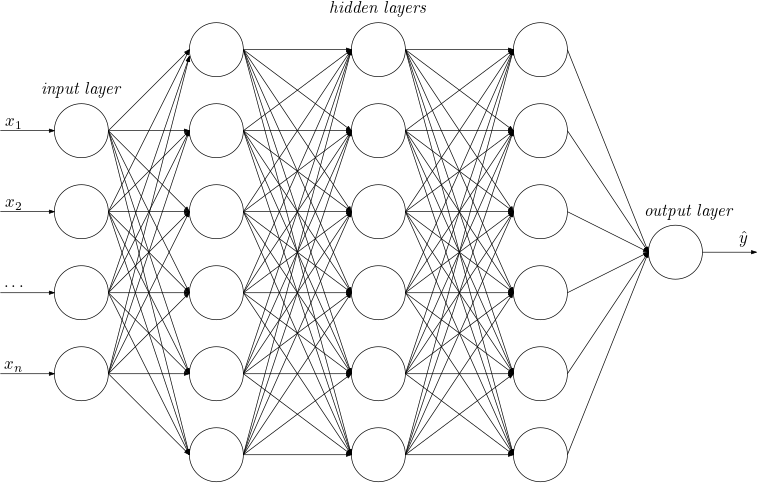
\includegraphics[width=12cm]{ffn.png}
    \caption{Fully connected Feed-forward Neural Network \cite{matous}}
    \label{fig:ffn}
\end{figure}

%=======================================================================================================================

\subsubsection{Cost Function}
Cost function $C(\vec{w})$ is used in ANN's training process. It takes all weights and biases of an ANN as its input, in the form of a vector $\vec{w}$ and calculates a single real number expressing ANN's incorrectness \cite{Goodfellow-et-al-2016}. The number is high when the ANN performs poorly and gets lower when the ANN's output gets closer to the correct result. The main goal of training is then to minimize the cost function. 

%=======================================================================================================================
\subsubsection{Backpropagation}
Backpropagation, short of backward propagation of errors, is a widely used algorithm in training FFN using \textit{gradient descent} to find a local minimum of a cost function and update ANN's weights \cite{birlliantbackprop}.

A gradient of a function with multiple variables gives us the direction of the steepest gradient ascent, where we should step to rapidly increase the output and find the local maximum. Naturally, its negative will point towards a local minimum. 

The usual practice is to divide training samples into small \textit{batches} of size $n$. We will calculate a gradient descent for each sample in the batch and use their average gradient descent to update the network's weights. The average gradient descent tells us which weights should be adjusted for the ANN to get closer to the correct results \cite{birlliantbackprop}.

\begin{equation}
    {- \gamma \nabla C(\vec{w}_i) + \vec{w}_i \rightarrow \vec{w}_{i+1} }
\end{equation}

Here, $\vec{w_i}$ is weights of the network at the current state (batch), $\vec{w_{i+1}}$ is updated weights, $\gamma$ is the learning rate and $-\nabla C(\vec{w_i})$ is the gradient descent.
